\documentclass[a4paper,1pt]{jsarticle}


% 数式
\usepackage{amsmath,amssymb,amsfonts}
\usepackage{bm}
% 画像
\usepackage[dvipdfmx]{graphicx}
\usepackage[dvipdfmx]{color}
\usepackage[dvipdfmx]{xcolor}
\usepackage{float}
\newcommand{\blue}[1]{\textcolor{blue}{#1}}



%テキストの表示領域の調節
\setlength{\textwidth}{\paperwidth}
\addtolength{\textwidth}{-40truemm}
\setlength{\textheight}{\paperheight}
\addtolength{\textheight}{-45truemm}

%余白の調節
\setlength{\topmargin}{-10.4truemm}
\setlength{\evensidemargin}{-5.4truemm}
\setlength{\oddsidemargin}{-5.4truemm}
\setlength{\headheight}{17pt}
\setlength{\headsep}{10mm}
\addtolength{\headsep}{-17pt}
\setlength{\footskip}{5mm}


\begin{document}
\section{目的}
resonance tubeにより音叉の振動数を測定すること.\\




\section{理論}

 \subsection*{算術平均の確率誤差}

 \begin{eqnarray}
  \label{kakuritugosa}
  r_a=\pm0.6745\sqrt{\dfrac{[v^2]}{n(n-1)}}
\end{eqnarray}

\begin{eqnarray}
  \label{kaisekizansa}
  [v^2]=\sum_{i=1}^n v_i^2=\sum_{i=1}^n(q_i-\bar{q})^2
\end{eqnarray}

\begin{eqnarray}
  \label{kaisekizansa}
  Q=F(q_i,q_2,...)
\end{eqnarray}


  $Q:,q_1,q_2,\dots\qquad の誤差をそれぞれ\qquad r:r_1,r_2,...\qquad として,$

  \begin{eqnarray}
    \label{kaisekizansa}
    r^2=\left(\frac{\partial F}{\partial q_1}r_1\right)^2+\left(\frac{\partial F}{\partial q_2}r_2\right)^2+\dots
  \end{eqnarray}


  


  $q_i:測定値,\; n:測定回数,\; \bar{q}:平均値$\\\\




\subsection*{振動数の導出}
$0{}^\circ{C},1気圧における空気中の音の速度をV_0とすると$\\

\begin{eqnarray}
  \label{velosity_0}
 V_0=\sqrt{\dfrac{\gamma p_0}{\rho _0}}=\sqrt{\dfrac{1.403\times 1.013\times 10^6}{331.4\times 10^2 }}=331.4\times 10^2[cm/sec]
\end{eqnarray}\\

$となる.ただし\gamma は空気の比熱比,p_0は標準気圧,\rho _0は空気の密度である.$\\

$実際に空気中を音が伝播する時には,その時の温度および湿度に対する補正を行わなければならない.$\\
$温度t[{}^\circ{C}],気圧p[hPa],水蒸気の分圧e[hPa]の時の伝播速度Vは,$\\

\begin{eqnarray}
  \label{velosity}
 V=V_0(1+0.00183t)\{1+(3/16)(e/p)\}=331.4\times 10^2(1+0.00183t)\{1+(3/16)(e/p)\}\qquad[cm/sec]
\end{eqnarray}\\

$で与えられる.$\\

$実験の便宜上同一種類の進行波と後退派との干渉により生ずる定常波(stationary\quad wave)を用いる.$\\

$図1のように下部に水面がある管中を音波が進行して定常波ができる場合,粗なる媒質より密なる媒質への反射面では筋(node)を生ずる.すなわち入射波と反射波との間に\pi radian(すなわち\lambda /2[cm])なる位相差を考えなければならないが逆に蜜より疎への反射面には腹(loop)を生ずるゆえ,位相差を考える必要はない.このような定常波の節間または腹間の距離は\lambda /2 [cm]に等しい.今昔の波長を\lambda [cm],振動数を\nu [sec^{-1}]とすれば$\\

\begin{eqnarray}
  \label{hz}
 \nu =V/\lambda \quad[Hz]
\end{eqnarray}\\

$となる関係がある.したがってVは(7)を用い,\lambda を測定して音叉の振動数\nu を計算することができる.$\\

\section{実験方法}



\begin{enumerate}
  \item 共鳴管ABの中に水を入れて水面が管口Aの近くに来るようにCを上げる.水面がAの近くに来た時Cの下のcockを閉じてCを下の方に置いていく.音叉をゴムハンマー(プラスチック)でたたいて管端に持って来ると同時にCの下のcockを開くと,水面は徐々に下って行くが音叉が水面上の気柱と共鳴する時には音が大きくなり共鳴の位置を知ることができる.
  \item 水面が最低位に来た時にCのcockを閉じてCを充分上の方に置き直す.
  \item 再び音叉を鳴らしながらCの下のcockを開き水面を上げて前と同様に共鳴点を求めていく.
  \item 同様の実験を繰り返して,その共鳴点の位置,$N_1,N_2,N_3,\dots を各2回読み取り各々y_1,y_2,\dots とする.$
  \item 別紙「連続して繰り返される測定」にしたがって共鳴時の波長$\lambda $を求めることができる.
  \item $室温t[{}^\circ{C}]$,大気圧p[hPa]および水蒸気の分圧e[hPa]を文末の表より知れば,(6)より,その時の音速Vを求めることができる.
  \item $\lambda とVが求まれば(6)にしたがってその音叉の振動数\nu が測定できる$
  \item 3種の音叉につき各音叉の振動数を求める.
\end{enumerate}

$\divideontimes 図2の上部に示すように定常波のloopは開口端Aと厳密には一致しない.今N_1より\lambda /4の点をとりL_0とすればL_0はAよりXだけ外になる.すなわちX=(\lambda /4)-AN_1であってXと管の半径rとの比を口端補正(terminal correction)と呼びこれを実験的に定めればX/r=0.55〜0.85となる.$\\

$\divideontimes 音叉の振動数は温度の上昇と共に少し減少する.0[{}^\circ{C}]およびt[{}^\circ{C}]における振動数を\nu _0,\nu とすれば\nu _0=\nu (1+0.000112t) によって求めた振動数を0[{}^\circ{C}]の振動数に書き直すこともできる.$\\

$\divideontimes 音叉はゴムハンマー(プラスチック)以外のもので叩いてはならない.硬いもので強く叩いて傷をつけると振動数に変化を生ずるし,強く叩いたことにより多くの倍音を生じて正しい音叉の基本音と混乱を生ずる.$



\clearpage

\begin{figure}[h]
  \begin{center}
  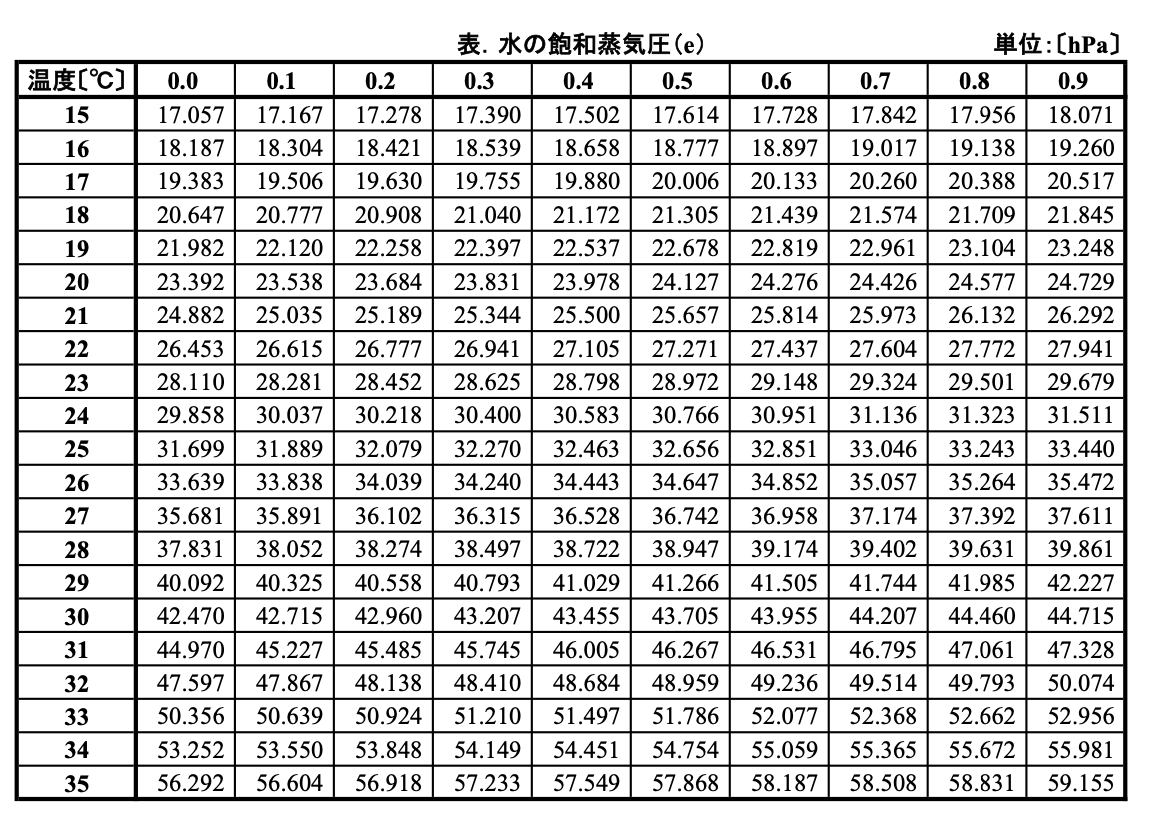
\includegraphics[width=130mm]{act1.png}
  \end{center}
\end{figure}

\begin{figure}[h]
  \begin{center}
  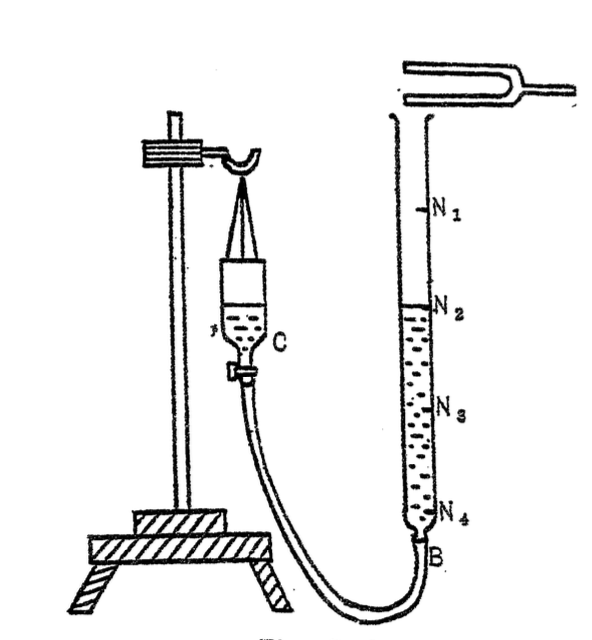
\includegraphics[width=100mm]{act2.png}
  \caption{実験装置概略図}
  \end{center}
\end{figure}

\begin{figure}[h]
  \begin{center}
  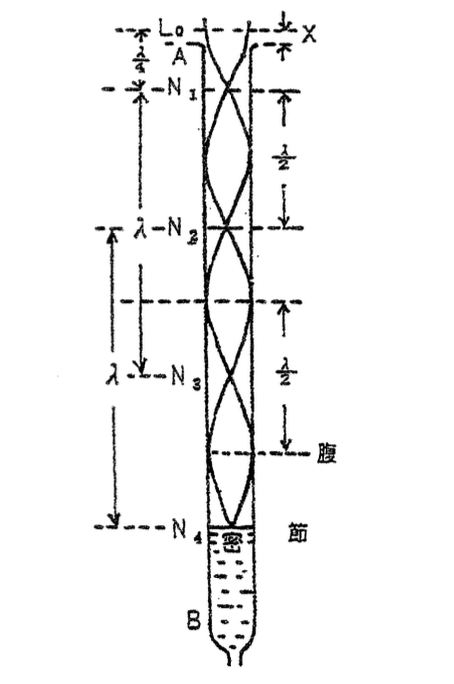
\includegraphics[width=100mm]{act3.png}
  \caption{開口端補正}
  \end{center}
\end{figure}

\clearpage

\section{データ処理・結果}

実験を行う前に,使用する管管に記載された150[cm]の目盛りと実際の長さとのスケールを計測することで,補正値を算出した.

\begin{table}[H]
  \caption{管の補正}
  \label{table:SpeedOfLight}
  \centering
  \begin{tabular}{|c||r|r|r|r|r|r|r|r|r|r|}
    \hline
    n & 実測値[cm] \\
    \hline\hline
    
    1 & 149.70 \\
    2 & 149.90 \\
    3 & 150.00 \\
    4 & 149.65 \\
    5 & 149.70 \\  

    \hline\hline
    Sum & 748.95 \\
    \hline
    Ave & 149.79 \\

    \hline
  \end{tabular}


\end{table}

$\dfrac{149.79}{150}=0.9986より,実測値に補正値0.9986をかけた補正後の値を用いて,波長を求める.$

\subsection[1]{音叉1(1400Hz)}

\subsection*{波長$\lambda$ の導出}

\begin{table}[H]
  \caption{共鳴点の測定値}
  \label{table:SpeedOfLight}
  \centering
  \begin{tabular}{|c||r|r|r|r|r|r|r|r|r|r|}
    \hline
    n & 1回目 [cm]& 2回目 [cm]& 平均値[cm] & 補正後$N_i$[cm] \\
    \hline\hline
    
    1 & 4.80 & 4.75 & 4.78 & 4.77 \\
    2 & 17.80 & 17.40 & 17.60 & 17.58 \\
    3 & 29.55 & 29.65 & 29.60 & 29.56 \\
    4 & 42.30 & 42.45 & 42.38 & 42.32 \\
    5 & 54.15 & 54.20 & 54.18 & 54.10 \\
    6 & 66.75 & 66.80 & 66.78 & 66.68 \\
    7 & 79.20 & 79.30 & 79.25 & 79.14 \\
    

    \hline
  \end{tabular}


\end{table}

$共鳴点の個数が奇数個であるため,桁数が揃っているN_2〜N_7のデータを用いて波長を以下のように算出する.$\\

\begin{table}[H]
  \caption{音叉の波長}
  \label{table:SpeedOfLight}
  \centering
  \begin{tabular}{|c||r|r|r|r|r|r|r|r|r|r|}
    \hline
     & $(3/2)\lambda =N_{i+3}-N_{i} [cm]$ & $\lambda [cm]$ & $v_\lambda $[cm]&  $v_\lambda ^2\times 10^4 [cm^2]$\\
    \hline\hline
    
   
    i=2 & 36.52 & 24.349 & -0.200 & 398.88078 \\
    i=3 & 37.12 & 24.749 & 0.200 & 398.88078 \\
    i=4 & 36.82 & 24.549 & 0.000 & 0.00000 \\
    

    \hline\hline

    Sum & & 73.647 & 0.000 & 797.76157 \\
    \hline
    Ave & & 24.549 &  &  \\
    \hline
  \end{tabular}


\end{table}

$よって\lambda の最確値は\lambda = 24.549 [cm].\\$

$確率誤差は理論(1)より,r_\lambda = \pm 0.6745\sqrt{\dfrac{797.76157\times 10^{-4}}{3\times 2}}=\pm 0.077776[cm].$

\subsection*{伝播速度Vの導出}

\begin{table}[H]
  \caption{温度t,気圧p,水蒸気の分圧eの測定値}
  \label{table:SpeedOfLight}
  \centering
  \begin{tabular}{|c||r|r|r|r|r|r|r|r|r|r|}
    \hline
    n & $t[{}^\circ{C}]$ & p[hPa] & e[hPa] \\
    \hline\hline
    
    
    1 & 23.8 & 1001.0 & 29.5010 \\
    2 & 23.8 & 1000.9 & 29.5010 \\
    3 & 23.6 & 1000.9 & 29.1480 \\
    4 & 23.5 & 1000.2 & 28.9720 \\
    5 & 23.5 & 1000.1 & 28.9720 \\

    \hline\hline
    Sum & 118.2 & 5003.1 & 146.0940 \\
    \hline
    Ave & 23.64 & 1000.6 & 29.21880 \\
    \hline
    

    \hline
  \end{tabular}




\end{table}

$表より,t,p,eの最確値はそれぞれ,t=23.64[{}^\circ{C}],\quad p=1000.6[hPa],\quad e=29.21880[hPa].$\\

$したがって理論(6)より,伝播速度Vの最確値は,$\\

$V=331.4\times 10^2(1+0.00183\times 23.64)\{1+(3/16)\times \dfrac{29.21880}{1000.6}\}=34762.97[cm/sec].$\\

\begin{table}[H]
  \caption{温度tの誤差}
  \label{table:SpeedOfLight}
  \centering
  \begin{tabular}{|c||r|r|r|r|r|r|r|r|r|r|}
    \hline
    n & $v_t[{}^\circ{C}]$ & $v_t^2\times 10^4[{}^\circ{C}^2]$ \\
    \hline\hline
    
    1 & 0.16 & 256.00000 \\
    2 & 0.16 & 256.00000 \\
    3 & -0.04 & 16.00000 \\
    4 & -0.14 & 196.00000 \\
    5 & -0.14 & 196.00000 \\
   
    
    \hline\hline
    Sum & 0.00 & 920.00000 \\
    \hline
  \end{tabular}


\end{table}

$よって理論(1)より,tの確率誤差r_tはr_t=\pm0.6745\sqrt{\dfrac{920.00000\times 10^{-4}}{5\times 4}}=\pm0.0457468[{}^\circ{C}].$\\

\begin{table}[H]
  \caption{気圧pの誤差}
  \label{table:SpeedOfLight}
  \centering
  \begin{tabular}{|c||r|r|r|r|r|r|r|r|r|r|}
    \hline
    n & $v_p[hPa]$ & $v_p^2\times 10^4[hPa]$ \\
    \hline\hline
    
    1 & 0.38 & 1444.00000 \\
    2 & 0.28 & 784.00000 \\
    3 & 0.28 & 784.00000 \\
    4 & -0.42 & 1764.00000 \\
    5 & -0.52 & 2704.00000 \\
    

   
    
    \hline\hline
    Sum & 0.00 & 7480.00000 \\
    \hline
  \end{tabular}


\end{table}

$よって理論(1)より,pの確率誤差r_pはr_p=\pm0.6745\sqrt{\dfrac{7480.00000\times 10^{-4}}{5\times 4}}=\pm0.1304421[hPa].$\\

\begin{table}[H]
  \caption{水蒸気の分圧eの誤差}
  \label{table:SpeedOfLight}
  \centering
  \begin{tabular}{|c||r|r|r|r|r|r|r|r|r|r|}
    \hline
    n & $v_e[hPa]$ & $v_e^2\times 10^4[hPa^2]$ \\
    \hline\hline
    
    1 & 0.28 & 796.36840 \\
    2 & 0.28 & 796.36840 \\
    3 & -0.07 & 50.12640 \\
    4 & -0.25 & 609.10240 \\
    5 & -0.25 & 609.10240 \\
    
   
    
    \hline\hline
    Sum & 0.00 & 2861.06800 \\
    \hline
  \end{tabular}


\end{table}

$よって理論(1)より,eの確率誤差r_eはr_e=\pm0.6745\sqrt{\dfrac{2861.06800\times 10^{-4}}{5\times 4}}=\pm0.0806735[hPa].$\\

$したがって理論(4)より,Vの確率誤差r_Vは,$\\

$r_V^2=\left(\dfrac{\partial V}{\partial t}r_t\right)^2+\left(\dfrac{\partial V}{\partial p}r_p\right)^2+\left(\dfrac{\partial V}{\partial e}r_e\right)^2=(2.789561)^2+(0.024677)^2+(0.522647)^2=8.055417 [(cm/sec)^2]$\\

$\therefore r_V=\pm2.838207[cm/sec].$

\subsection*{振動数$\nu $の導出}

$理論(7)より,振動数\nu の最確値は\nu =\dfrac{V}{\lambda }=\dfrac{34762.97}{24.549}=1416.07[Hz].$\\

$確率誤差r_\nu は理論(4)より,$\\

$r_\nu ^2=\left(\dfrac{\partial \nu }{\partial V}r_V \right)^2+\left(\dfrac{\partial \nu }{\partial \lambda }r_\lambda \right)^2=(0.115614)^2+(4.486370)^2=20.140885[Hz^2]$\\

$\therefore r_\nu = \pm 4.487860[Hz].$\\

$\therefore \nu =1416.07\pm4.487860=(1.416\pm0.004)\times10^3[Hz].$

\subsection[2]{音叉2(1600Hz)}

\subsection*{波長$\lambda$ の導出}

\begin{table}[H]
  \caption{共鳴点の測定値}
  \label{table:SpeedOfLight}
  \centering
  \begin{tabular}{|c||r|r|r|r|r|r|r|r|r|r|}
    \hline
    n & 1回目 [cm]& 2回目 [cm]& 平均値[cm] & 補正後$N_i$[cm] \\
    \hline\hline
    
    1 & 4.25 & 4.20 & 4.23 & 4.22 \\
    2 & 14.65 & 14.70 & 14.68 & 14.65 \\
    3 & 25.90 & 25.80 & 25.85 & 25.81 \\
    4 & 36.55 & 36.55 & 36.55 & 36.50 \\
    5 & 47.45 & 47.55 & 47.50 & 47.43 \\
    6 & 58.25 & 58.30 & 58.28 & 58.19 \\
    7 & 68.75 & 68.85 & 68.80 & 68.70 \\
    8 & 79.80 & 79.90 & 79.85 & 79.74 \\
    
    

    \hline
  \end{tabular}


\end{table}

\begin{table}[H]
  \caption{音叉の波長}
  \label{table:SpeedOfLight}
  \centering
  \begin{tabular}{|c||r|r|r|r|r|r|r|r|r|r|}
    \hline
    & $2\lambda =N_{i+4}-N_{i} [cm]$ & $\lambda [cm]$ & $v_\lambda $[cm]&  $v_\lambda ^2\times 10^6[cm^2]$\\
    \hline\hline
    
   
    i=1 & 43.21 &21.607& -0.003 & 9.738300 \\
    i=2 & 43.54 &21.769& 0.159 & 25329.319316 \\
    i=3 & 42.89 &21.445& -0.165 & 27354.885797 \\
    i=4 & 43.24 &21.620& 0.009 & 87.644704 \\
    
    
   
    
    

    \hline\hline

    Sum & & 86.441 & 0.000 & 52781.588117 \\
    \hline
    Ave & & 21.610 &  &  \\
    \hline
  \end{tabular}


\end{table}

$よって\lambda の最確値は\lambda = 21.610[cm].\\$

$確率誤差は理論(1)より,r_\lambda = \pm 0.6745\sqrt{\dfrac{52781.588117\times 10^{-6}}{4\times 3}}=\pm 0.044733[cm].$

\subsection*{伝播速度Vの導出}

\begin{table}[H]
  \caption{温度t,気圧p,水蒸気の分圧eの測定値}
  \label{table:SpeedOfLight}
  \centering
  \begin{tabular}{|c||r|r|r|r|r|r|r|r|r|r|}
    \hline
    n & $t[{}^\circ{C}]$ & p[hPa] & e[hPa] \\
    \hline\hline
    
    
    1 & 23.4 & 1000.1 & 28.7980 \\
    2 & 23.3 & 1000.1 & 28.6250 \\
    3 & 23.3 & 1000.1 & 28.6250 \\
    4 & 23.2 & 1000.1 & 28.4520 \\
    5 & 23.1 & 1000.2 & 28.2810 \\
    
    
    \hline\hline
    Sum & 116.3 & 5000.6 & 142.781 \\
    \hline
    Ave & 23.26 & 1000.1 & 28.5562 \\
    \hline
    

    \hline
  \end{tabular}




\end{table}

$表より,t,p,eの最確値はそれぞれ,t=23.26[{}^\circ{C}],\quad p=1000.1[hPa],\quad e=28.5562[hPa].$\\

$したがって理論(6)より,伝播速度Vの最確値は,$\\

$V=331.4\times 10^2(1+0.00183\times 23.26)\{1+(3/16)\times \dfrac{28.5562}{1000.1}\}=34735.60[cm/sec].$\\

\begin{table}[H]
  \caption{温度tの誤差}
  \label{table:SpeedOfLight}
  \centering
  \begin{tabular}{|c||r|r|r|r|r|r|r|r|r|r|}
    \hline
    n & $v_t[{}^\circ{C}]$ & $v_t^2\times 10^4[{}^\circ{C}^2]$ \\
    \hline\hline
    
    1 & 0.14 & 196.00000 \\
    2 & 0.04 & 16.00000 \\
    3 & 0.04 & 16.00000 \\
    4 & -0.06 & 36.00000 \\
    5 & -0.16 & 256.00000 \\
    

    
    \hline\hline
    Sum & 0.00 & 520.00000 \\
    \hline
  \end{tabular}


\end{table}

$よって理論(1)より,tの確率誤差r_tはr_t=\pm0.6745\sqrt{\dfrac{520.00000\times 10^{-4}}{5\times 4}}=\pm0.0343929[{}^\circ{C}].$\\

\begin{table}[H]
  \caption{気圧pの誤差}
  \label{table:SpeedOfLight}
  \centering
  \begin{tabular}{|c||r|r|r|r|r|r|r|r|r|r|}
    \hline
    n & $v_p[hPa]$ & $v_p^2\times 10^4[hPa]$ \\
    \hline\hline
    
    1 & -0.02 & 4.00000 \\
    2 & -0.02 & 4.00000 \\
    3 & -0.02 & 4.00000 \\
    4 & -0.02 & 4.00000 \\
    5 & 0.08 & 64.00000 \\
    

    

   
    
    \hline\hline
    Sum & 0.00 & 80.00000 \\
    \hline
  \end{tabular}


\end{table}

$よって理論(1)より,pの確率誤差r_pはr_p=\pm0.6745\sqrt{\dfrac{80.00000\times 10^{-4}}{5\times 4}}=\pm0.0134900[hPa].$\\

\begin{table}[H]
  \caption{水蒸気の分圧eの誤差}
  \label{table:SpeedOfLight}
  \centering
  \begin{tabular}{|c||r|r|r|r|r|r|r|r|r|r|}
    \hline
    n & $v_e[hPa]$ & $v_e^2\times 10^4[hPa^2]$ \\
    \hline\hline
    
    1 & 0.24 & 584.67240 \\
    2 & 0.07 & 47.33440 \\
    3 & 0.07 & 47.33440 \\
    4 & -0.10 & 108.57640 \\
    5 & -0.28 & 757.35040 \\
   

   
    
    \hline\hline
    Sum & 0.00 & 1545.26800 \\
    \hline
  \end{tabular}


\end{table}

$よって理論(1)より,eの確率誤差r_eはr_e=\pm0.6745\sqrt{\dfrac{1545.26800\times 10^{-4}}{5\times 4}}=\pm0.0592883[hPa].$\\

$したがって理論(4)より,Vの確率誤差r_Vは,$\\

$r_V^2=\left(\dfrac{\partial V}{\partial t}r_t\right)^2+\left(\dfrac{\partial V}{\partial p}r_p\right)^2+\left(\dfrac{\partial V}{\partial e}r_e\right)^2=(2.096965)^2+(0.002495)^2+(0.384038)^2=4.544751 [(cm/sec)^2]$\\

$\therefore r_V=\pm2.131842[cm/sec].$

\subsection*{振動数$\nu $の導出}

$理論(7)より,振動数\nu の最確値は\nu =\dfrac{V}{\lambda }=\dfrac{34735.60}{21.610}=1607.36[Hz].$\\

$確率誤差r_\nu は理論(4)より,$\\

$r_\nu ^2=\left(\dfrac{\partial \nu }{\partial V}r_V \right)^2+\left(\dfrac{\partial \nu }{\partial \lambda }r_\lambda \right)^2=(0.098649)^2+(3.327244)^2=11.080285[Hz^2]$\\

$\therefore r_\nu = \pm 3.328706[Hz].$\\

$\therefore \nu =1607.36\pm3.328706=(1.607\pm0.003)\times10^3[Hz].$





\subsection[3]{音叉3(1800Hz)}

\subsection*{波長$\lambda$ の導出}

\begin{table}[H]
  \caption{共鳴点の測定値}
  \label{table:SpeedOfLight}
  \centering
  \begin{tabular}{|c||r|r|r|r|r|r|r|r|r|r|}
    \hline
    n & 1回目 [cm]& 2回目 [cm]& 平均値[cm] & 補正後$N_i$[cm] \\
    \hline\hline
    
    1 & 3.75 & 3.85 & 3.80 & 3.79 \\
    2 & 12.55 & 12.60 & 12.58 & 12.56 \\
    3 & 22.65 & 22.75 & 22.70 & 22.67 \\
    4 & 32.80 & 32.30 & 32.55 & 32.50 \\
    5 & 42.25 & 42.40 & 42.33 & 42.27 \\
    6 & 51.90 & 51.90 & 51.90 & 51.83 \\
    7 & 61.70 & 61.95 & 61.83 & 61.74 \\
    8 & 71.35 & 71.45 & 71.40 & 71.30 \\
    
    
    

    \hline
  \end{tabular}


\end{table}


\begin{table}[H]
  \caption{音叉の波長}
  \label{table:SpeedOfLight}
  \centering
  \begin{tabular}{|c||r|r|r|r|r|r|r|r|r|r|}
    \hline
    & $2\lambda =N_{i+4}-N_{i} [cm]$ & $\lambda [cm]$ & $v_\lambda $[cm]&  $v_\lambda ^2\times 10^4[cm^2]$\\
    \hline\hline
    
   
    i=1 &38.47 & 19.236 & -0.215 & 463.640482 \\
    i=2 &39.27 & 19.635 & 0.184 & 338.990237 \\
    i=3 &39.07 & 19.535 & 0.084 & 70.992210 \\
    i=4 &38.80 & 19.398 & -0.053 & 28.143688 \\
    
    
    
    

    \hline\hline

    Sum &&77.803 & 0.000 & 901.766616 \\
    \hline
    Ave & &19.451 &  &  \\
    \hline
  \end{tabular}


\end{table}

$よって\lambda の最確値は\lambda = 19.451[cm].\\$

$確率誤差は理論(1)より,r_\lambda = \pm 0.6745\sqrt{\dfrac{901.766616\times 10^{-4}}{4\times 3}}=\pm 0.058471[cm].$

\subsection*{伝播速度Vの導出}

\begin{table}[H]
  \caption{温度t,気圧p,水蒸気の分圧eの測定値}
  \label{table:SpeedOfLight}
  \centering
  \begin{tabular}{|c||r|r|r|r|r|r|r|r|r|r|}
    \hline
    n & $t[{}^\circ{C}]$ & p[hPa] & e[hPa] \\
    \hline\hline
    
    
    1 & 23.1 & 1000.2 & 28.2810 \\
    2 & 23.1 & 1000.3 & 28.2810 \\
    3 & 23.2 & 1000.2 & 28.4520 \\
    4 & 23.4 & 1000.1 & 28.7980 \\
    5 & 23.5 & 1000.1 & 28.9720 \\
    
    

    \hline\hline
    Sum & 116.3 & 5000.9 & 142.784 \\
    \hline
    Ave & 23.26 & 1000.2 & 28.5568 \\
    \hline
    

    \hline
  \end{tabular}




\end{table}

$表より,t,p,eの最確値はそれぞれ,t=23.26[{}^\circ{C}],\quad p=1000.2[hPa],\quad e=28.5568[hPa].$\\

$したがって理論(6)より,伝播速度Vの最確値は,$\\

$V=331.4\times 10^2(1+0.00183\times 23.26)\{1+(3/16)\times \dfrac{28.5568}{1000.2}\}=34735.60[cm/sec].$\\

\begin{table}[H]
  \caption{温度tの誤差}
  \label{table:SpeedOfLight}
  \centering
  \begin{tabular}{|c||r|r|r|r|r|r|r|r|r|r|}
    \hline
    n & $v_t[{}^\circ{C}]$ & $v_t^2\times 10^4[{}^\circ{C}^2]$ \\
    \hline\hline
    
    1 & -0.16 & 256.00000 \\
    2 & -0.16 & 256.00000 \\
    3 & -0.06 & 36.00000 \\
    4 & 0.14 & 196.00000 \\
    5 & 0.24 & 576.00000 \\
    

   
    
    \hline\hline
    Sum & 0.00 & 1320.00000 \\
    \hline
  \end{tabular}


\end{table}

$よって理論(1)より,tの確率誤差r_tはr_t=\pm0.6745\sqrt{\dfrac{1320.00000\times 10^{-4}}{5\times 4}}=\pm0.0547966[{}^\circ{C}].$\\

\begin{table}[H]
  \caption{気圧pの誤差}
  \label{table:SpeedOfLight}
  \centering
  \begin{tabular}{|c||r|r|r|r|r|r|r|r|r|r|}
    \hline
    n & $v_p[hPa]$ & $v_p^2\times 10^4[hPa]$ \\
    \hline\hline
    
    1 & 0.02 & 4.00000 \\
    2 & 0.12 & 144.00000 \\
    3 & 0.02 & 4.00000 \\
    4 & -0.08 & 64.00000 \\
    5 & -0.08 & 64.00000 \\
    

   
    
    \hline\hline
    Sum & 0.00 & 280.00000 \\
    \hline
  \end{tabular}


\end{table}

$よって理論(1)より,pの確率誤差r_pはr_p=\pm0.6745\sqrt{\dfrac{280.00000\times 10^{-4}}{5\times 4}}=\pm0.0252375[hPa].$\\

\begin{table}[H]
  \caption{水蒸気の分圧eの誤差}
  \label{table:SpeedOfLight}
  \centering
  \begin{tabular}{|c||r|r|r|r|r|r|r|r|r|r|}
    \hline
    n & $v_e[hPa]$ & $v_e^2\times 10^4[hPa^2]$ \\
    \hline\hline
    
    1 & -0.28 & 760.65640 \\
    2 & -0.28 & 760.65640 \\
    3 & -0.10 & 109.83040 \\
    4 & 0.24 & 581.77440 \\
    5 & 0.42 & 1723.91040 \\
    

    
   
    
    \hline\hline
    Sum & 0.00 & 3936.82800 \\
    \hline
  \end{tabular}


\end{table}

$よって理論(1)より,eの確率誤差r_eはr_e=\pm0.6745\sqrt{\dfrac{3936.82800\times 10^{-4}}{5\times 4}}=\pm0.0946325[hPa].$\\

$したがって理論(4)より,Vの確率誤差r_Vは,$\\

$r_V^2=\left(\dfrac{\partial V}{\partial t}r_t\right)^2+\left(\dfrac{\partial V}{\partial p}r_p\right)^2+\left(\dfrac{\partial V}{\partial e}r_e\right)^2=(3.340999)^2+(0.004667)^2+(0.612942)^2=11.537991 [(cm/sec)^2]$\\

$\therefore r_V=\pm3.396762[cm/sec].$

\subsection*{振動数$\nu $の導出}

$理論(7)より,振動数\nu の最確値は\nu =\dfrac{V}{\lambda }=\dfrac{34735.60}{19.451}=1785.81[Hz].$\\

$確率誤差r_\nu は理論(4)より,$\\

$r_\nu ^2=\left(\dfrac{\partial \nu }{\partial V}r_V \right)^2+\left(\dfrac{\partial \nu }{\partial \lambda }r_\lambda \right)^2=(0.174633)^2+(5.368287)^2=28.849003[Hz^2]$\\

$\therefore r_\nu = \pm 5.371127[Hz].$\\

$\therefore \nu =1785.81\pm5.371127=(1.786\pm0.005)\times10^3[Hz].$








\section{考察}

音叉1〜3までの振動数を算出したが,それぞれの算出された値と公称値の誤差率は以下のようになった.\\

\begin{table}[H]
  \caption{音叉1〜3の振動数の公称値との誤差率}
  \label{table:SpeedOfLight}
  \centering
  \begin{tabular}{c|r}
    
    音叉 & 誤差率[\%]\\
    \hline
    
    1 & +0.8〜1.4 \\
    2 & +0.3〜0.6 \\
    3 & -0.5〜1.0 \\
    
    

    
   
  \end{tabular}


\end{table}

この表より,3つとも概ね同じ精度で実験をできていると考えられる.また,音叉1に関しては,計算の都合上,共鳴点のデータをひとつ省いてしまっているため,(表2,表3参照)誤差率が他の2つよりも大きくなっていると考えられる.\\

また,この実験では温度,湿度,気圧を計測し,伝播速度Vを求めたが,$\nu $の確率誤差の誤差伝播の式からも分かるとおり,$\nu $の誤差はVよりも$\lambda $に大きく左右されるため,上表の誤差の原因は共鳴点測定時における個人差や人的要因が大きいと考える.




\end{document}